\documentclass[11pt,aspectratio=169]{beamer}

\usepackage[utf8]{inputenc}
\usepackage{lmodern}
\usepackage[english]{babel}
\usepackage{amssymb}
\usepackage{graphicx}
\usepackage{hyperref}
\usepackage{xcolor}
\usepackage{tikz}
\usepackage{amsmath}
\usepackage{csquotes}

\usepackage{caption} 
\usepackage{booktabs}
\usepackage{adjustbox}
\usepackage{subcaption} % for subfigures
\DeclareCaptionLabelSeparator{custom}{ -- }
\captionsetup[figure]{labelformat=simple, labelsep=custom, name=Figure}
\usepackage{amsfonts}
\usepackage{listings}

% Links to other files
\graphicspath{{figures/}}

\newcommand{\manualcite}[1]{\textcolor{gray}{\small[#1]}}


% Beamer template customisation
\beamertemplatenavigationsymbolsempty
\setbeamertemplate{page number in head/foot}[totalframenumber] % numéros de slides
\setbeamercovered{transparent}
\usetheme{Madrid}
\usecolortheme{default}

% Setup colors title page + footline
% \definecolor{deepblue}{RGB}{0, 50, 100} 
\definecolor{deepblue}{RGB}{140, 0, 51} 
\definecolor{roose}{RGB}{226, 0, 122}
\definecolor{gold}{rgb}{1.0, 0.84, 0.0}
\definecolor{silver}{rgb}{0.75, 0.75, 0.75}
\setbeamercolor{title}{bg=deepblue, fg=white} 
\setbeamercolor{frametitle}{bg=deepblue, fg=white}
\setbeamercolor{footline}{bg=deepblue, fg=white}
\setbeamercolor{author in head/foot}{bg=deepblue, fg=white} 
\setbeamercolor{title in head/foot}{bg=deepblue, fg=white} 
\setbeamercolor{date in head/foot}{bg=deepblue, fg=white}

% No more bold font in footline
\setbeamerfont{author in head/foot}{series=\normalfont}
\setbeamerfont{title in head/foot}{series=\normalfont}
\setbeamerfont{date in head/foot}{series=\normalfont} 
\setbeamerfont{footline}{series=\normalfont} 

% To cite papers manually
\newcommand{\mycitation}[1]{\textcolor{gray}{\small[#1]}}

% TITLEPAGE
\author[Barbara Gendron]{\large Barbara Gendron-Audebert, PhD student (MosAIk team)}
\title[Mastering LLM Fine-Tuning]{\huge Mastering Large Language Models: Efficient Techniques for Fine-Tuning}
\date{January 15, 2025}
\institute[DeepLorIA tutorial]{\large LORIA, Université de Lorraine, CNRS\\ DeepLorIA Network}
% {LORIA, Université de Lorraine, CNRS}

\begin{document}

\begin{frame}[plain]
    \vspace*{5pt}
    \begin{center}
        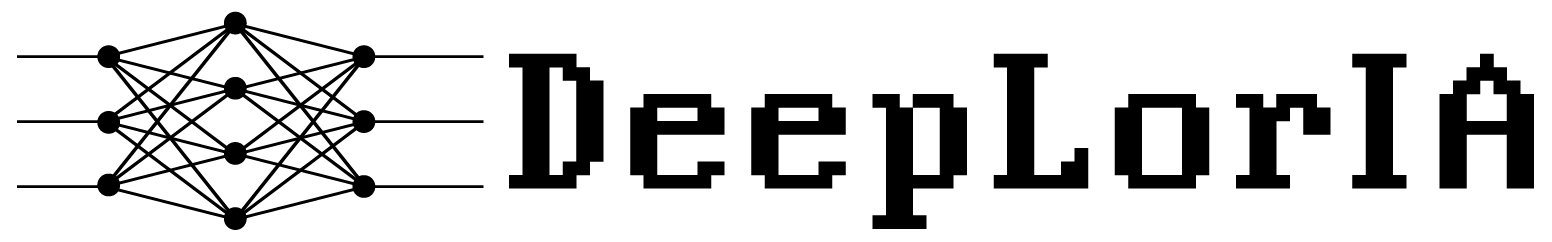
\includegraphics[scale=0.35]{DeepLorIA_logo1.png}
    \end{center}
    % \vspace*{5pt}
    \titlepage
\end{frame}

\section{Motivations}

\begin{frame}{About Me}
\begin{center}
    2nd-year PhD student - Knowledge-Enhanced Language Models (Université de Lorraine)
\end{center}
\vspace*{10pt}
Background \& Research
    \begin{itemize}
        \item Maths engineering degree
        \item Master Thesis: Meta-Learning in Conversational Context
        \item PhD Topic: Controlled Conversational Models through Conversation-Dedicated Ontology
        \item \textsl{Keywords: Large Language Models (LLMs), Conversational Agents, Ontologies, Fine-Tuning}
    \end{itemize}

% I study how to adapt the usual fine-tuning procedures to integrate external knowledge from an ontology. My PhD also require to build this external knowledge, so I have to develop a full, end-to-end hybridization pipeline between LLMs and Ontologies. 
% Hence, I developed several fine-tuning procedures for my research at Loria.
More info: \url{b-gendron.github.io}
\end{frame}

\section{Context}

\begin{frame}{Context}

\end{frame}

\begin{frame}{Recurrent Models for NLP (1)}
    
\end{frame}

\begin{frame}{Recurrent Models for NLP (2)}
    
\end{frame}

\begin{frame}{The Transformer Model}
    
\end{frame}

\begin{frame}{Attention Principle}
    
\end{frame}

\begin{frame}{From Transformer-Based Models to Large Language Models (LLMs)}
% The liberty of building behind enc only, dec only, enc dec, which structure for which application
% Very rich range of models and possible applications, even multimodal but I'm not dealing with that in this tutorial
\end{frame}

% slide un peu meta, piste de réflexion et d'ouverture pour close la partie
\begin{frame}{What Use-Cases of LLMs?}
    
\end{frame}

\section{Inside a Decoder-Based LLM}

\begin{frame}{Inside a Decoder-Based LLM}
    \begin{figure}
        \centering
        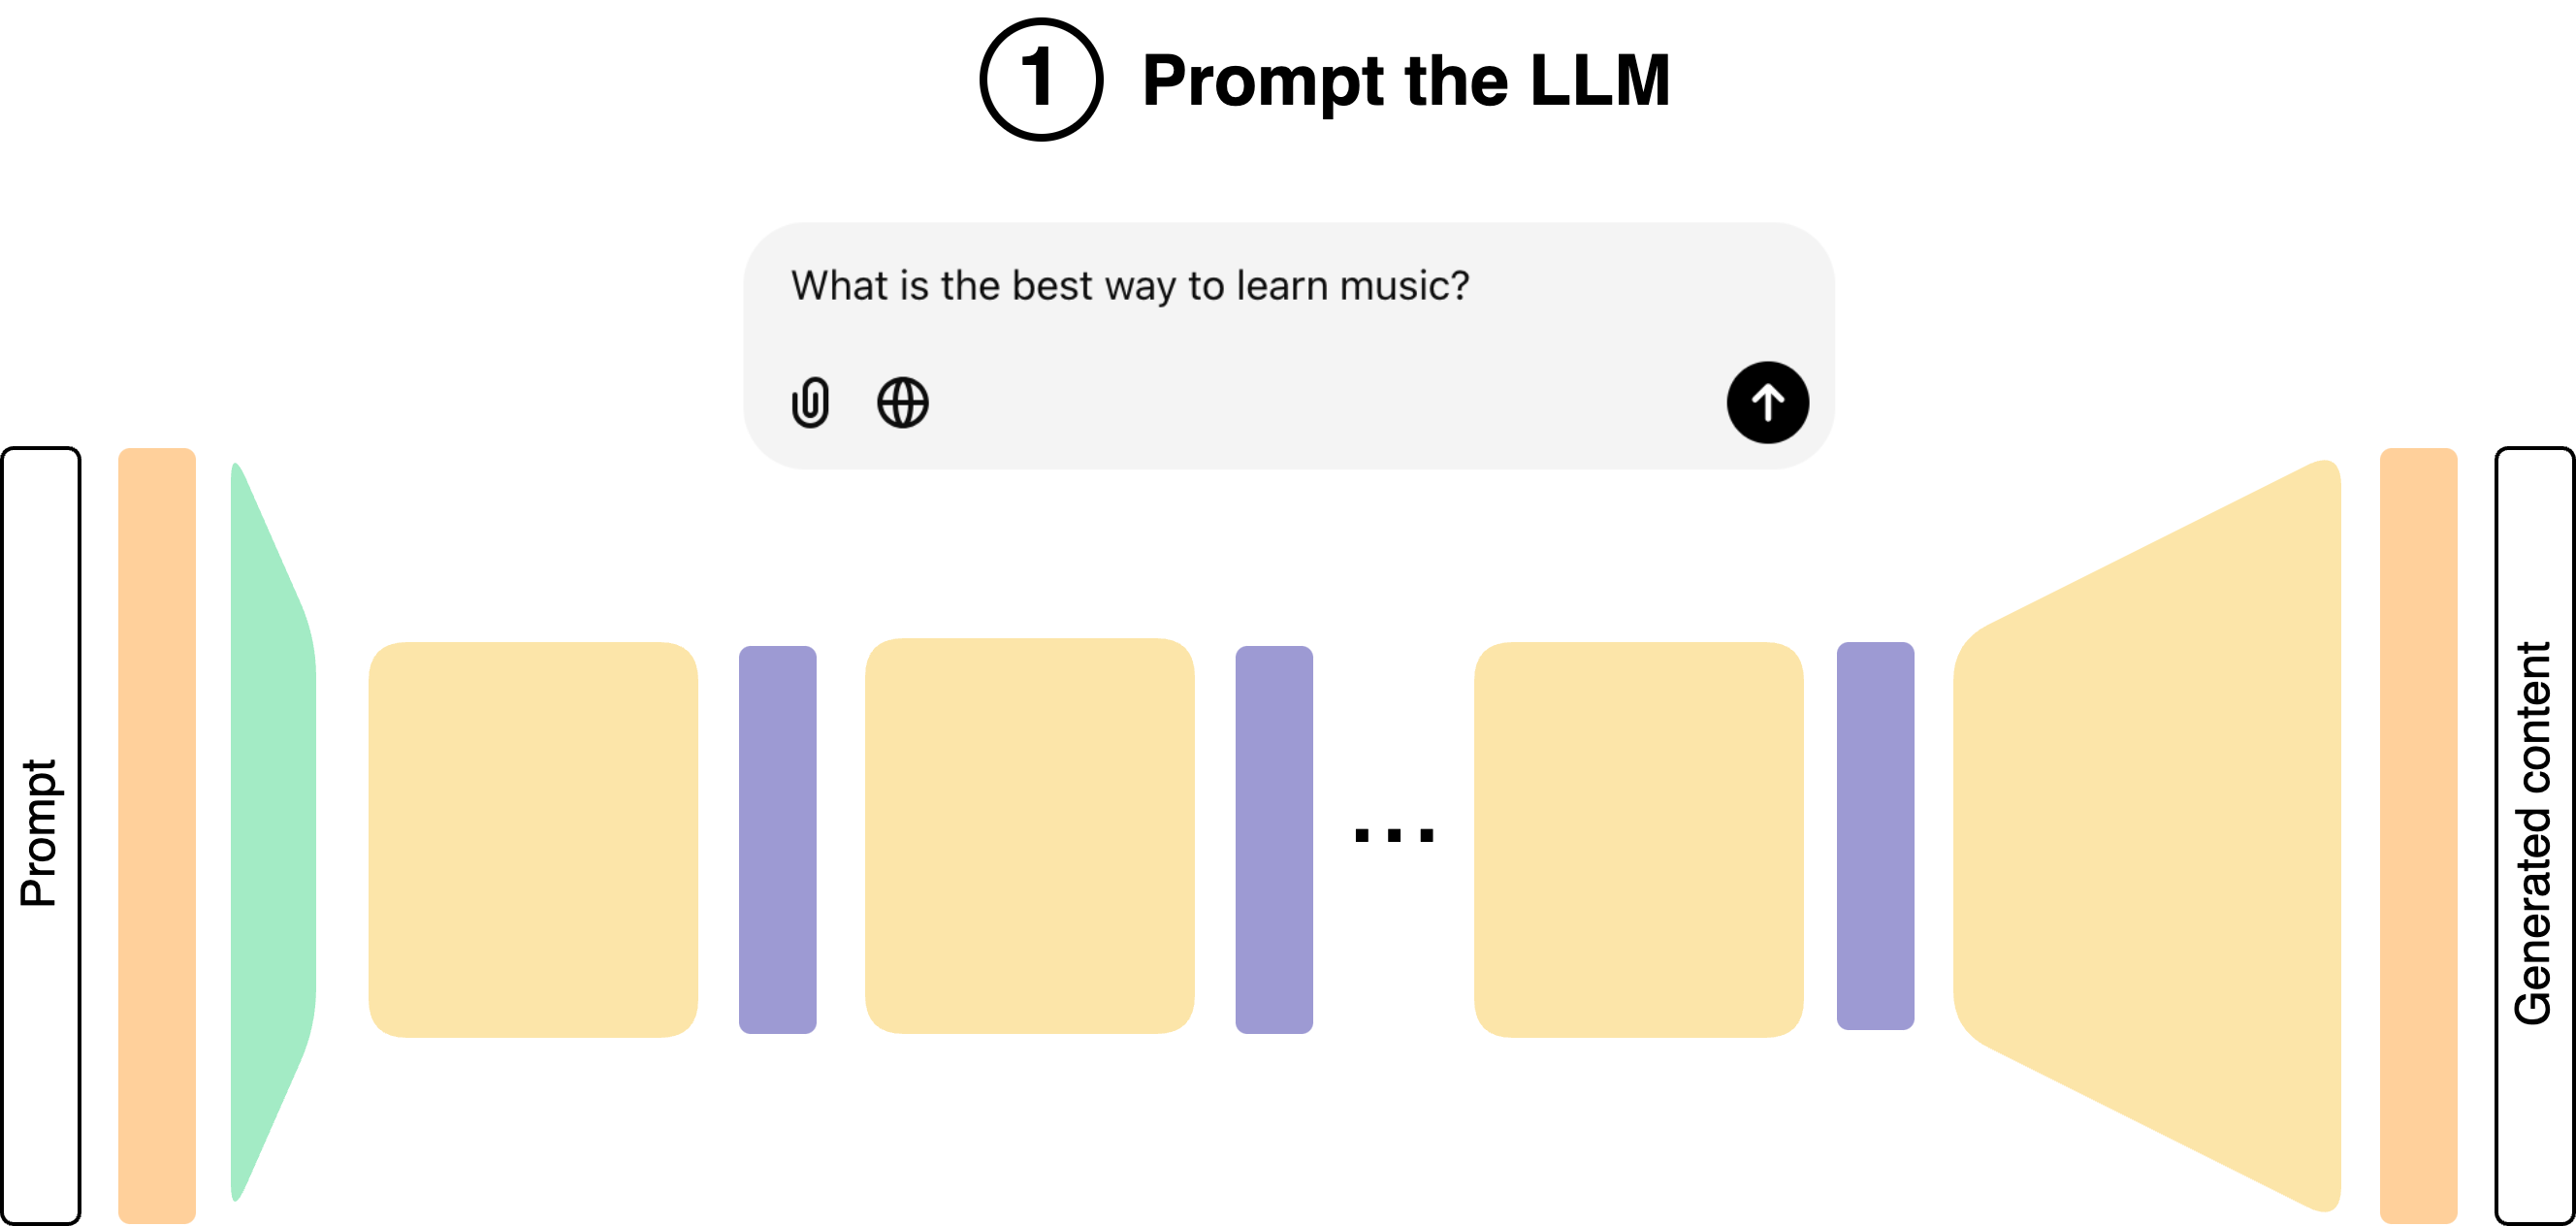
\includegraphics[width=0.95\textwidth]{llm_1.png}
    \end{figure}
\end{frame}

\begin{frame}{Inside a Decoder-Based LLM}
    \begin{figure}
        \centering
        \includegraphics[width=0.95\textwidth]{llm_2.png}
    \end{figure}
\end{frame}

\begin{frame}{Inside a Decoder-Based LLM}
    \begin{figure}
        \centering
        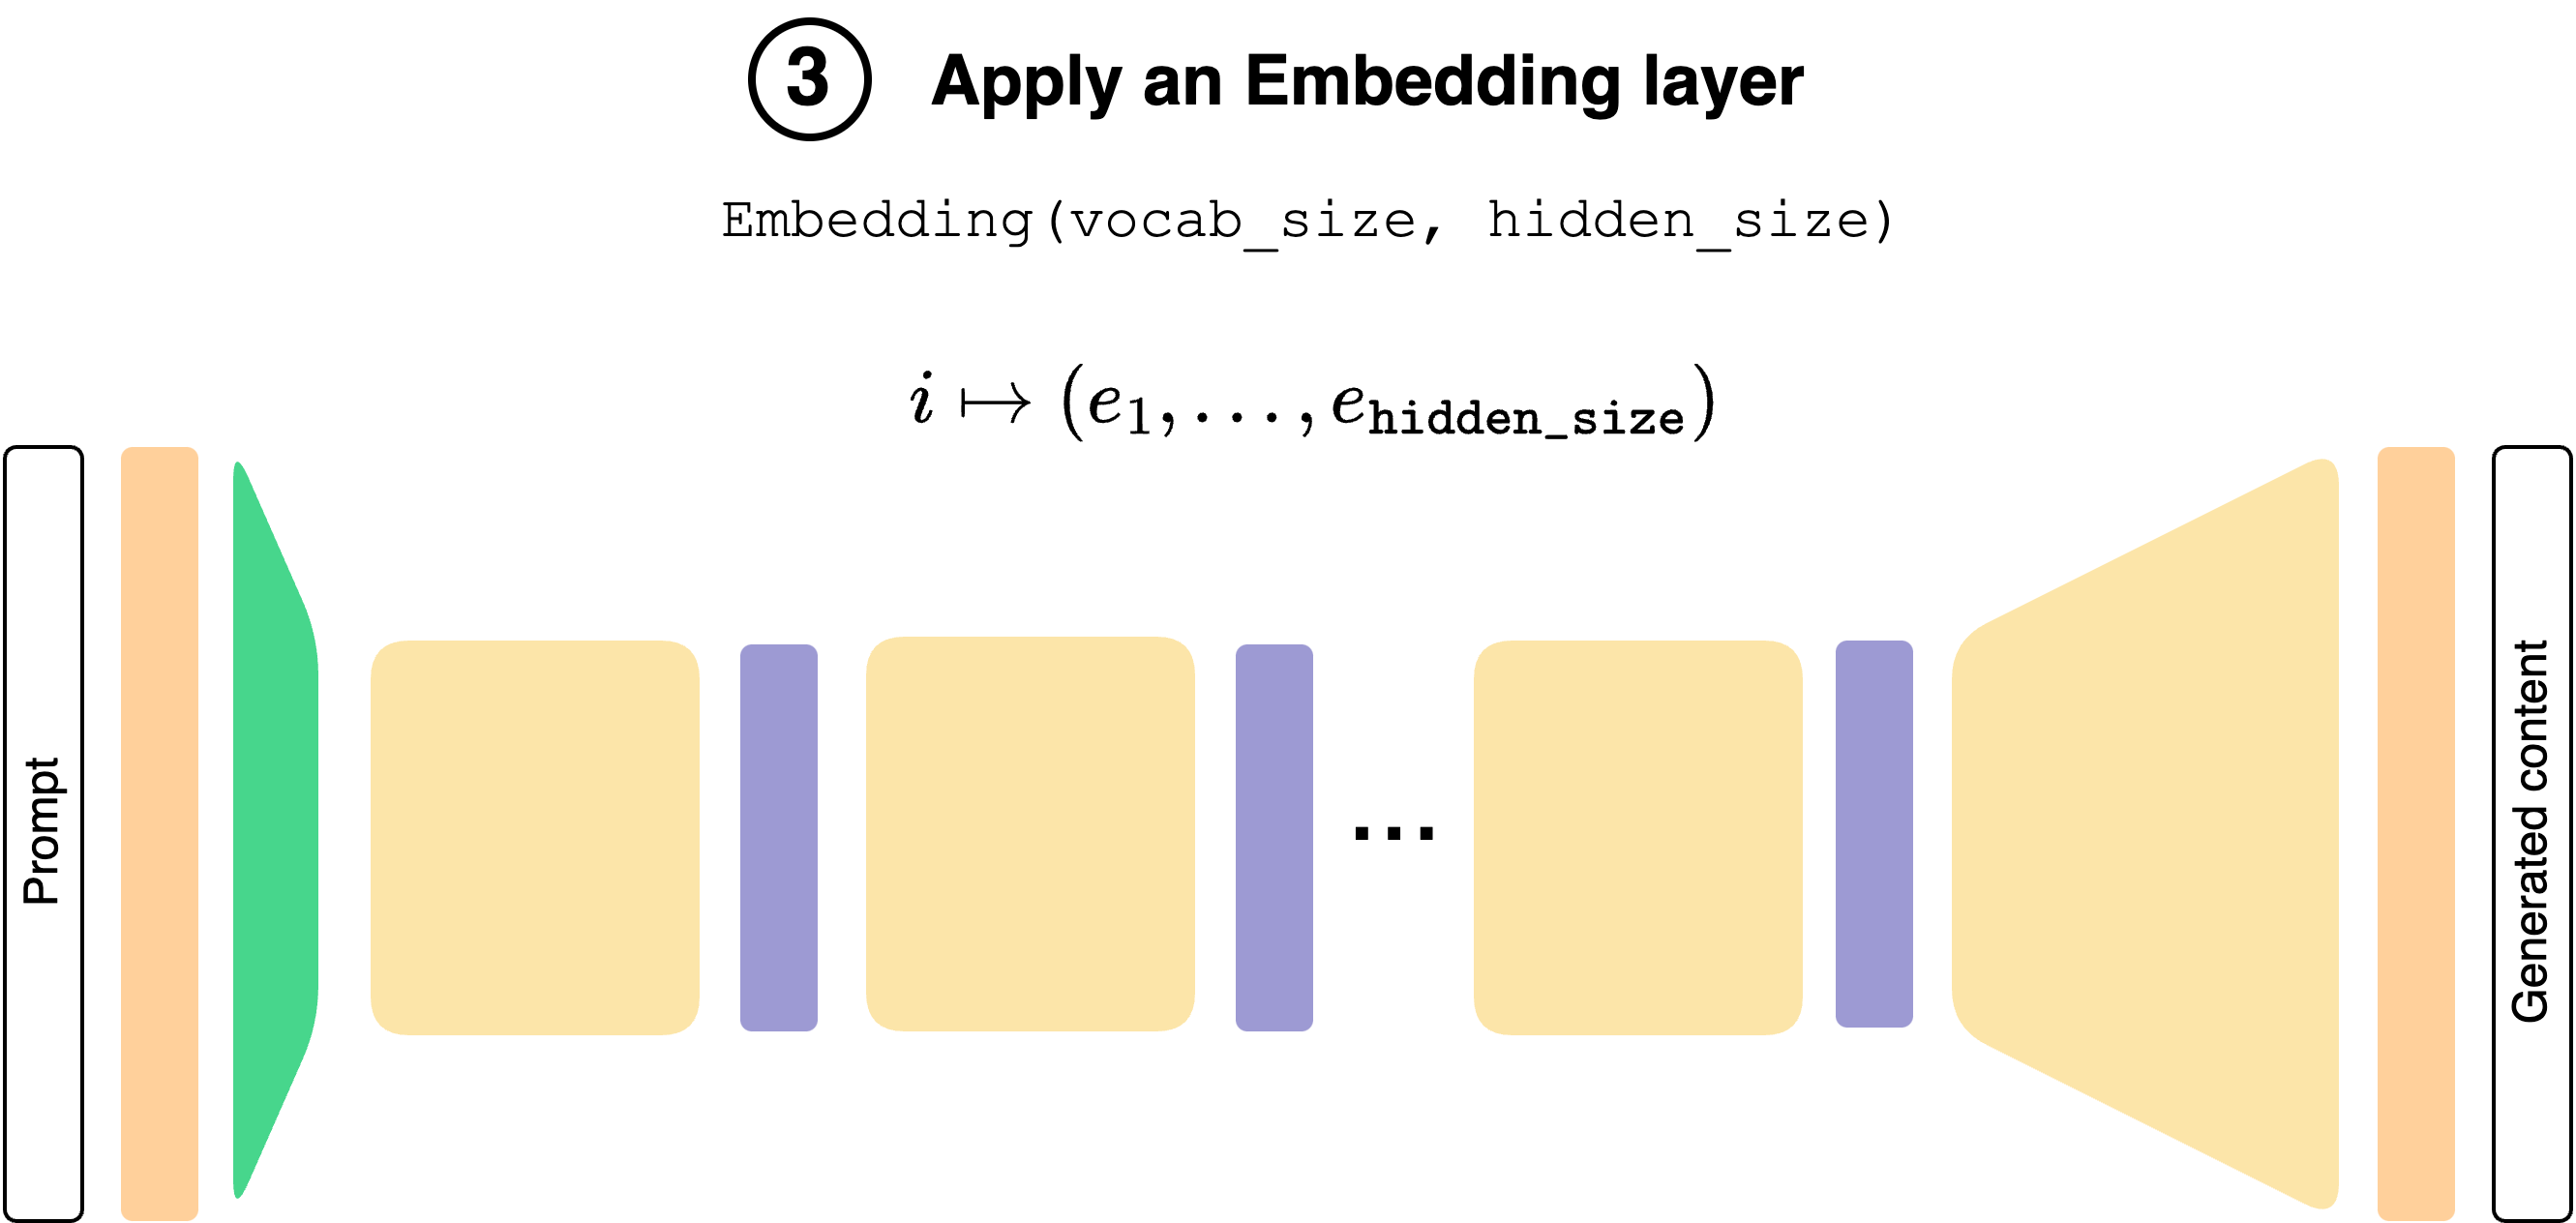
\includegraphics[width=0.95\textwidth]{llm_3.png}
    \end{figure}
\end{frame}

\begin{frame}{Inside a Decoder-Based LLM}
    \begin{figure}
        \centering
        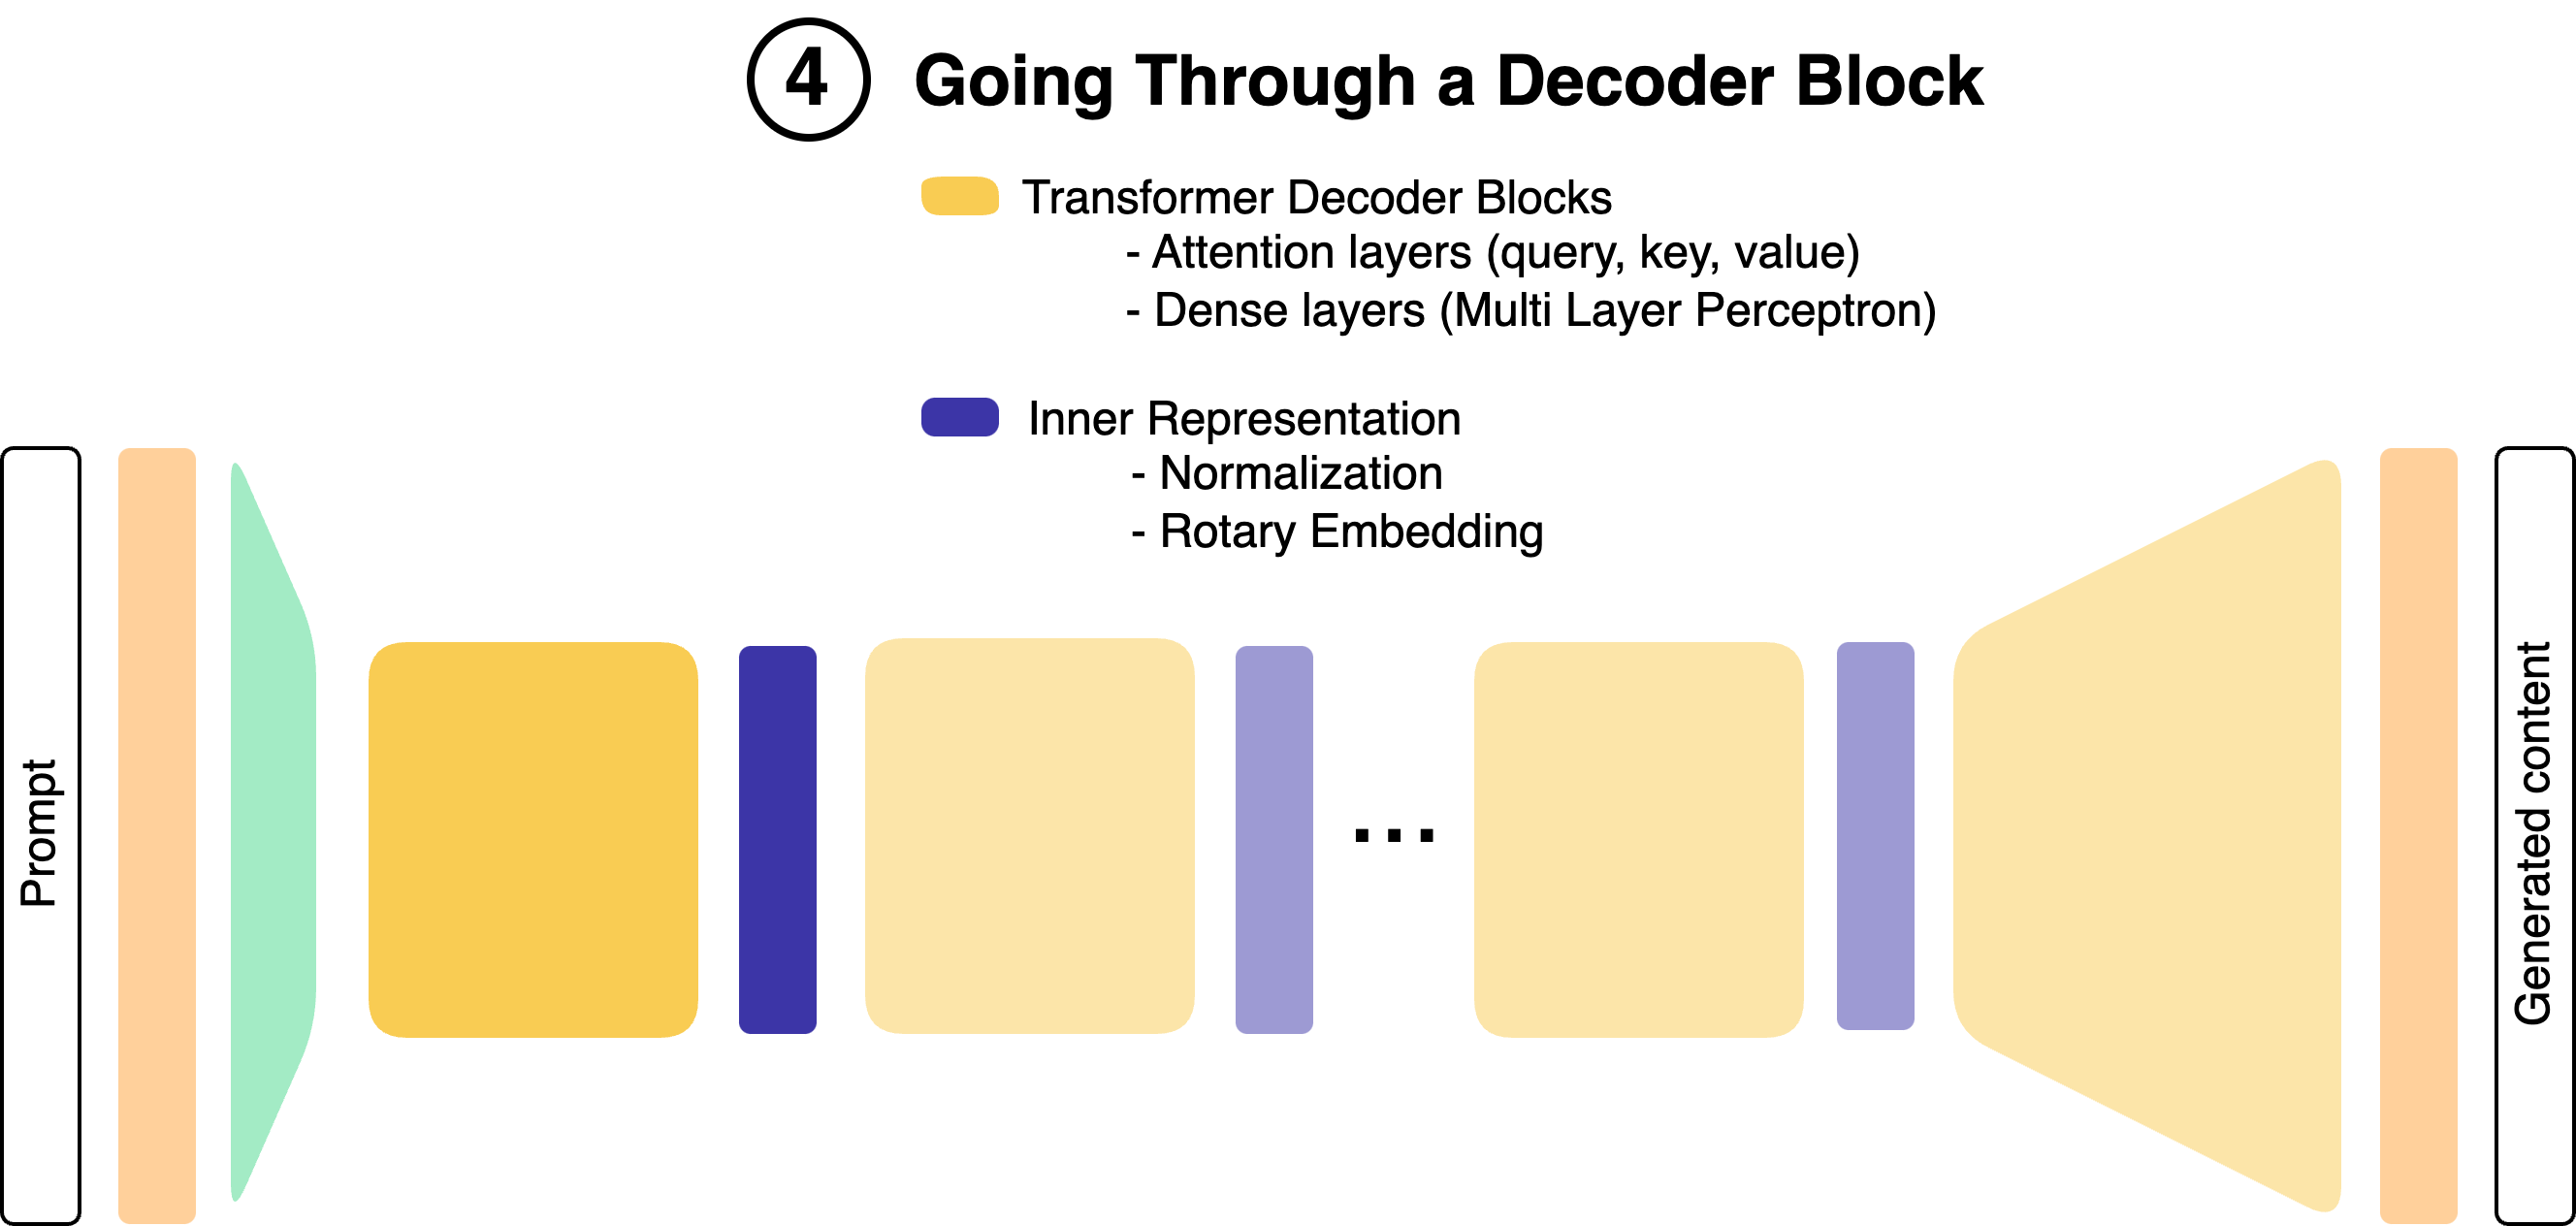
\includegraphics[width=0.95\textwidth]{llm_4.png}
    \end{figure}
\end{frame}

\begin{frame}{Inside a Decoder-Based LLM}
    \begin{figure}
        \centering
        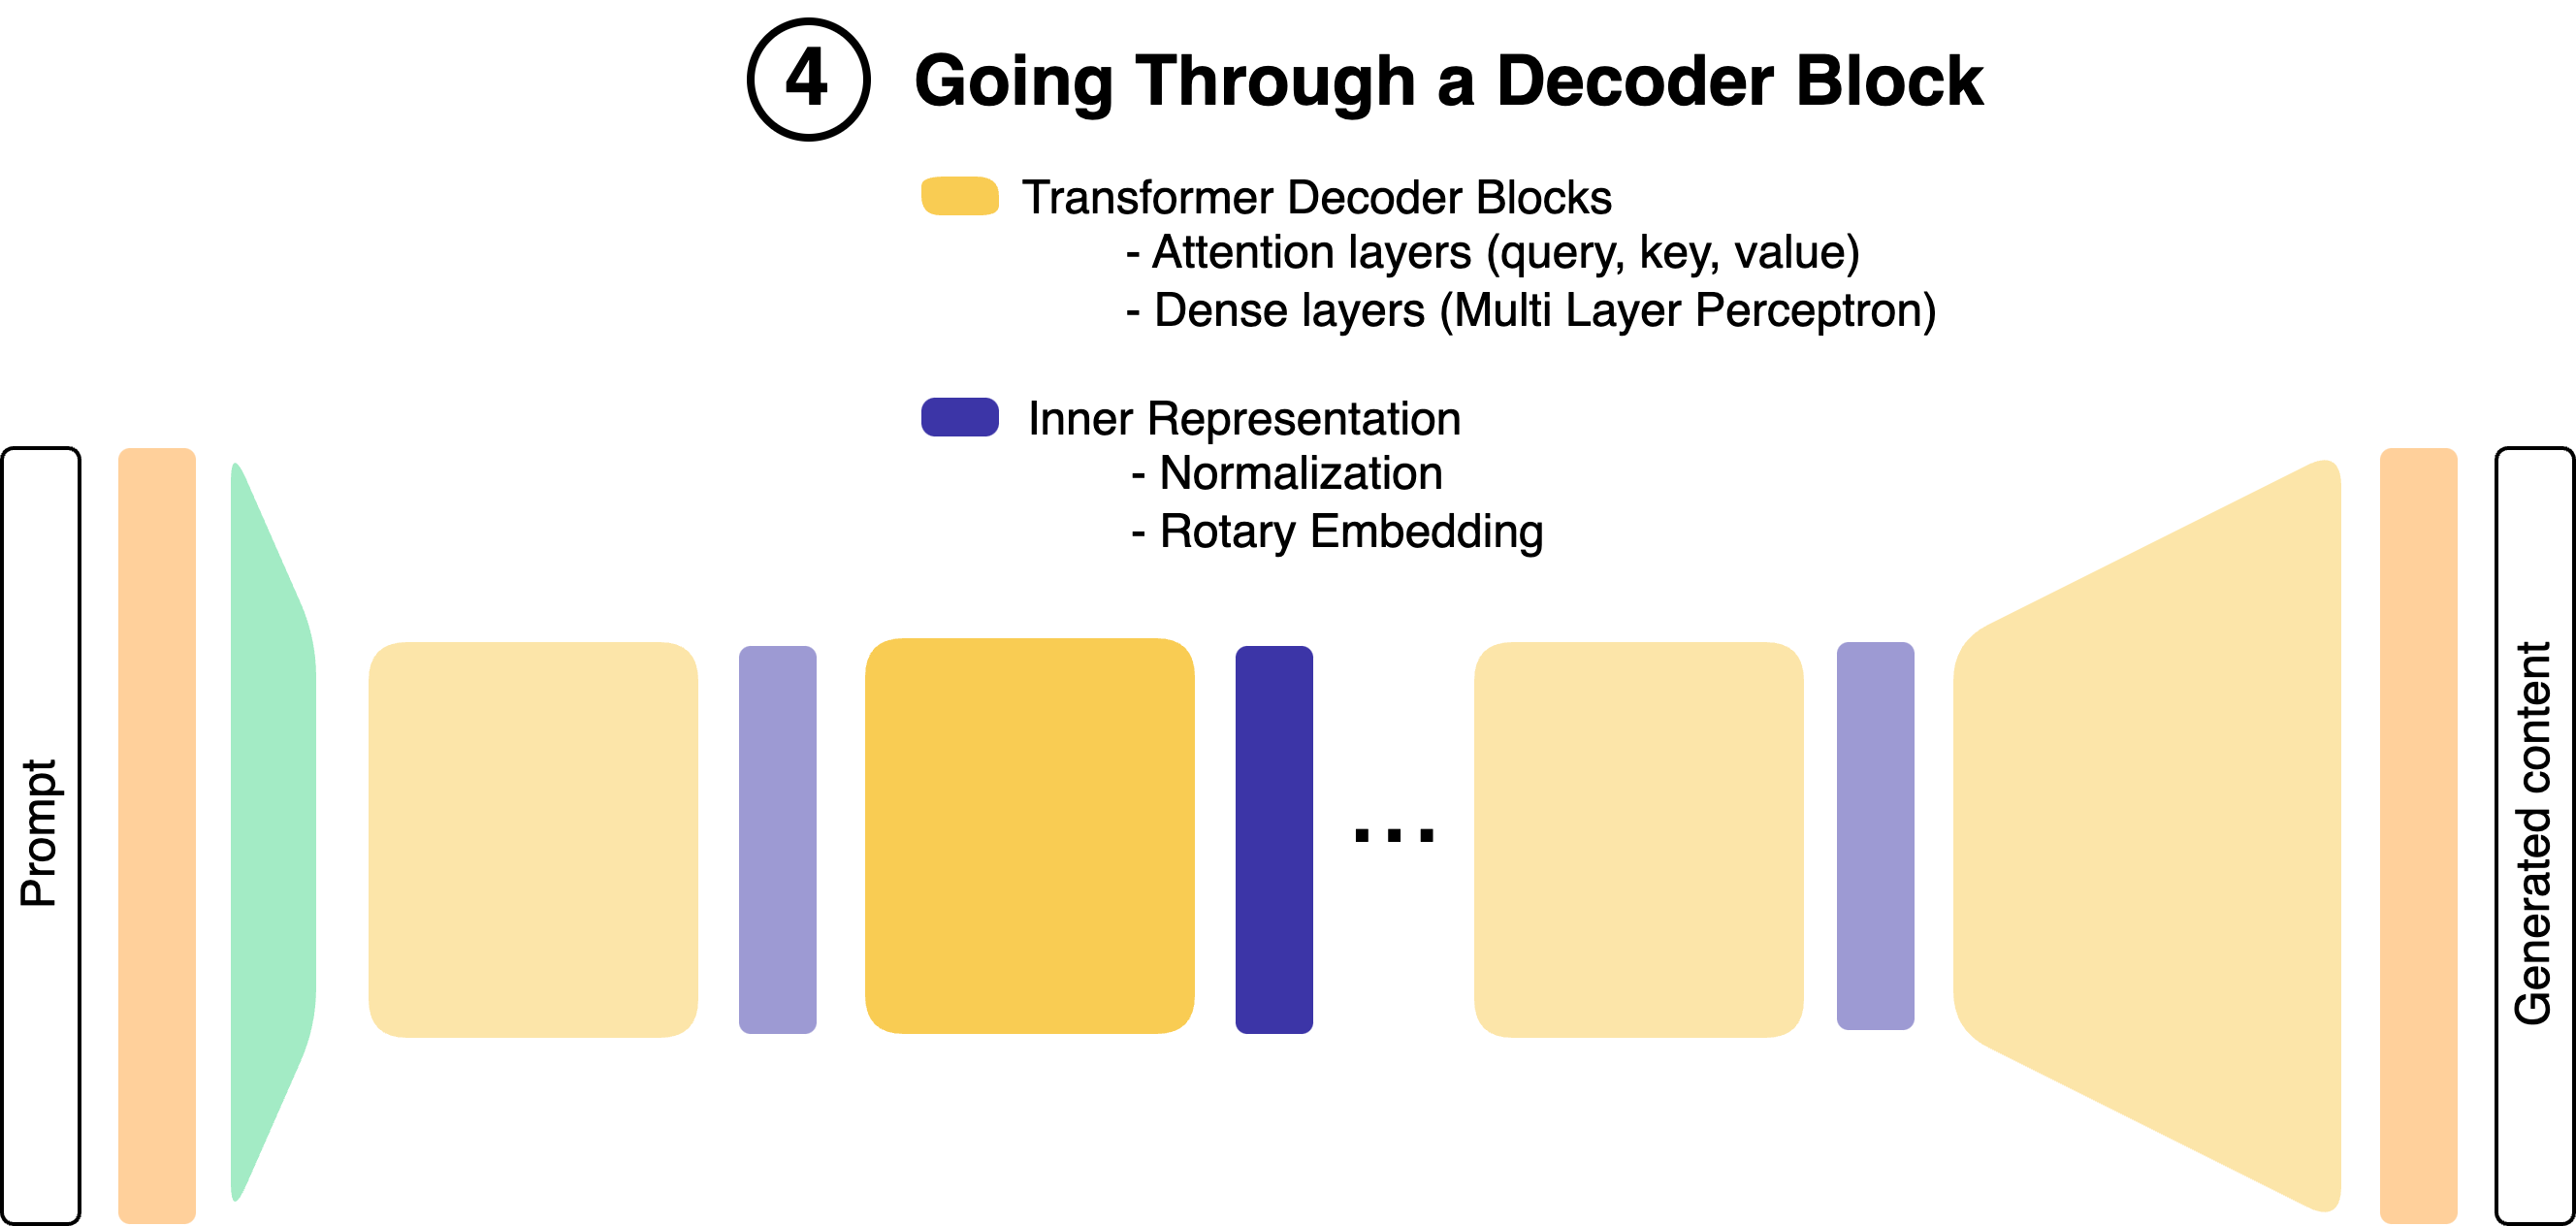
\includegraphics[width=0.95\textwidth]{llm_5.png}
    \end{figure}
\end{frame}

\begin{frame}{Inside a Decoder-Based LLM}
    \begin{figure}
        \centering
        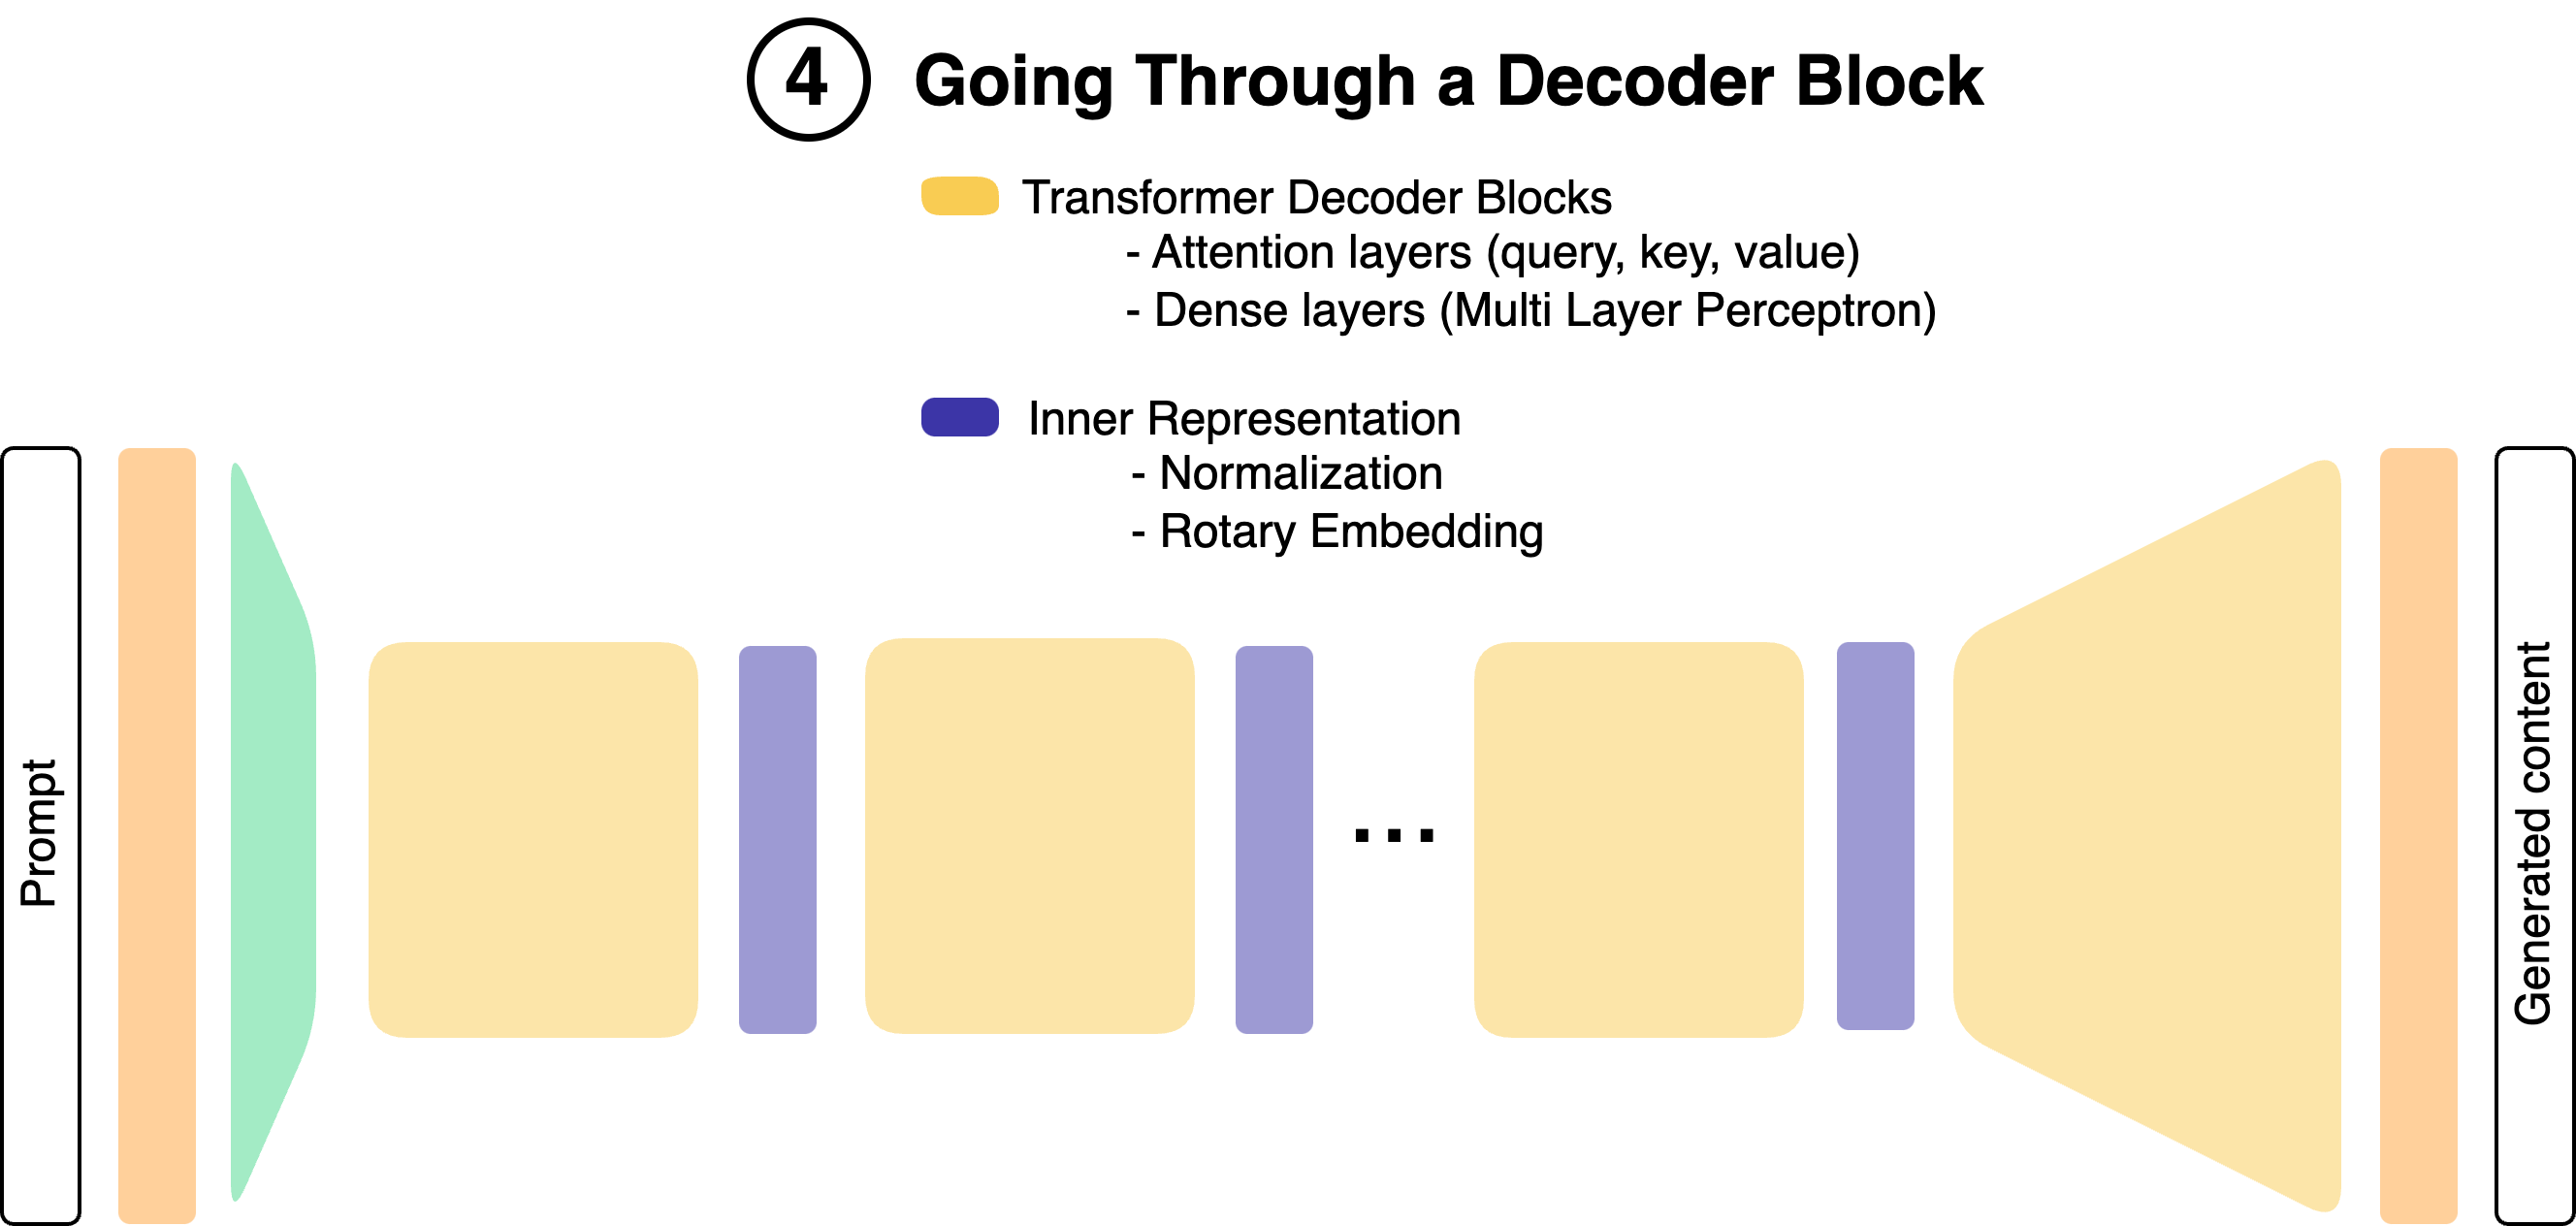
\includegraphics[width=0.95\textwidth]{llm_6.png}
    \end{figure}
\end{frame}

\begin{frame}{Inside a Decoder-Based LLM}
    \begin{figure}
        \centering
        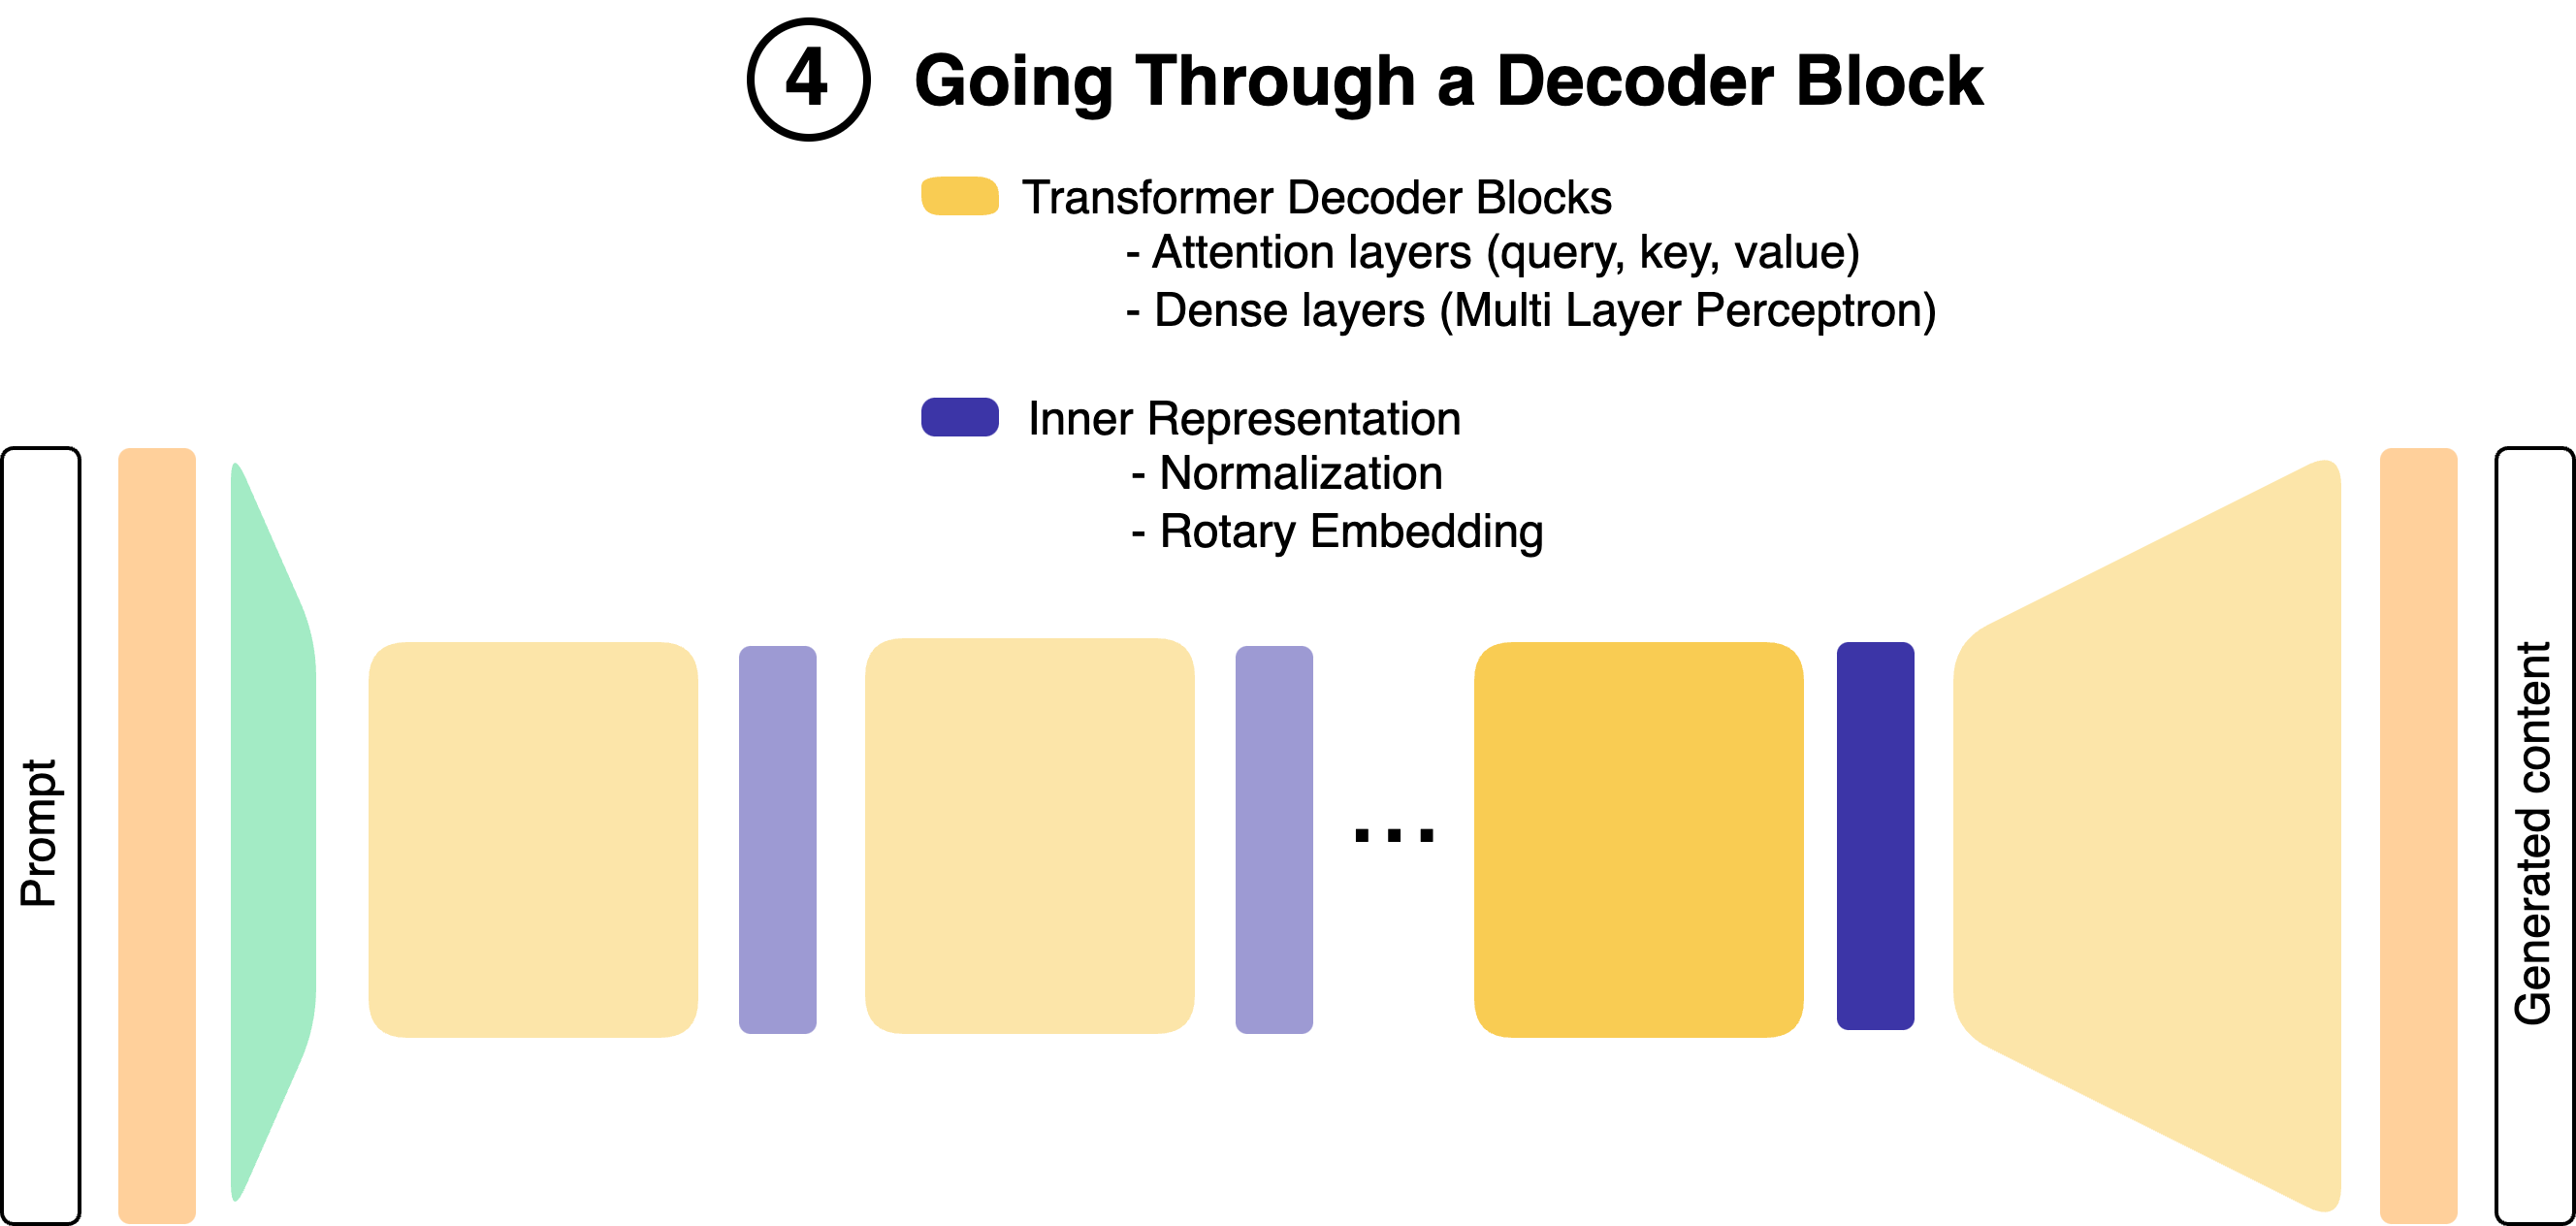
\includegraphics[width=0.95\textwidth]{llm_7.png}
    \end{figure}
\end{frame}

\begin{frame}{Inside a Decoder-Based LLM}
    \begin{figure}
        \centering
        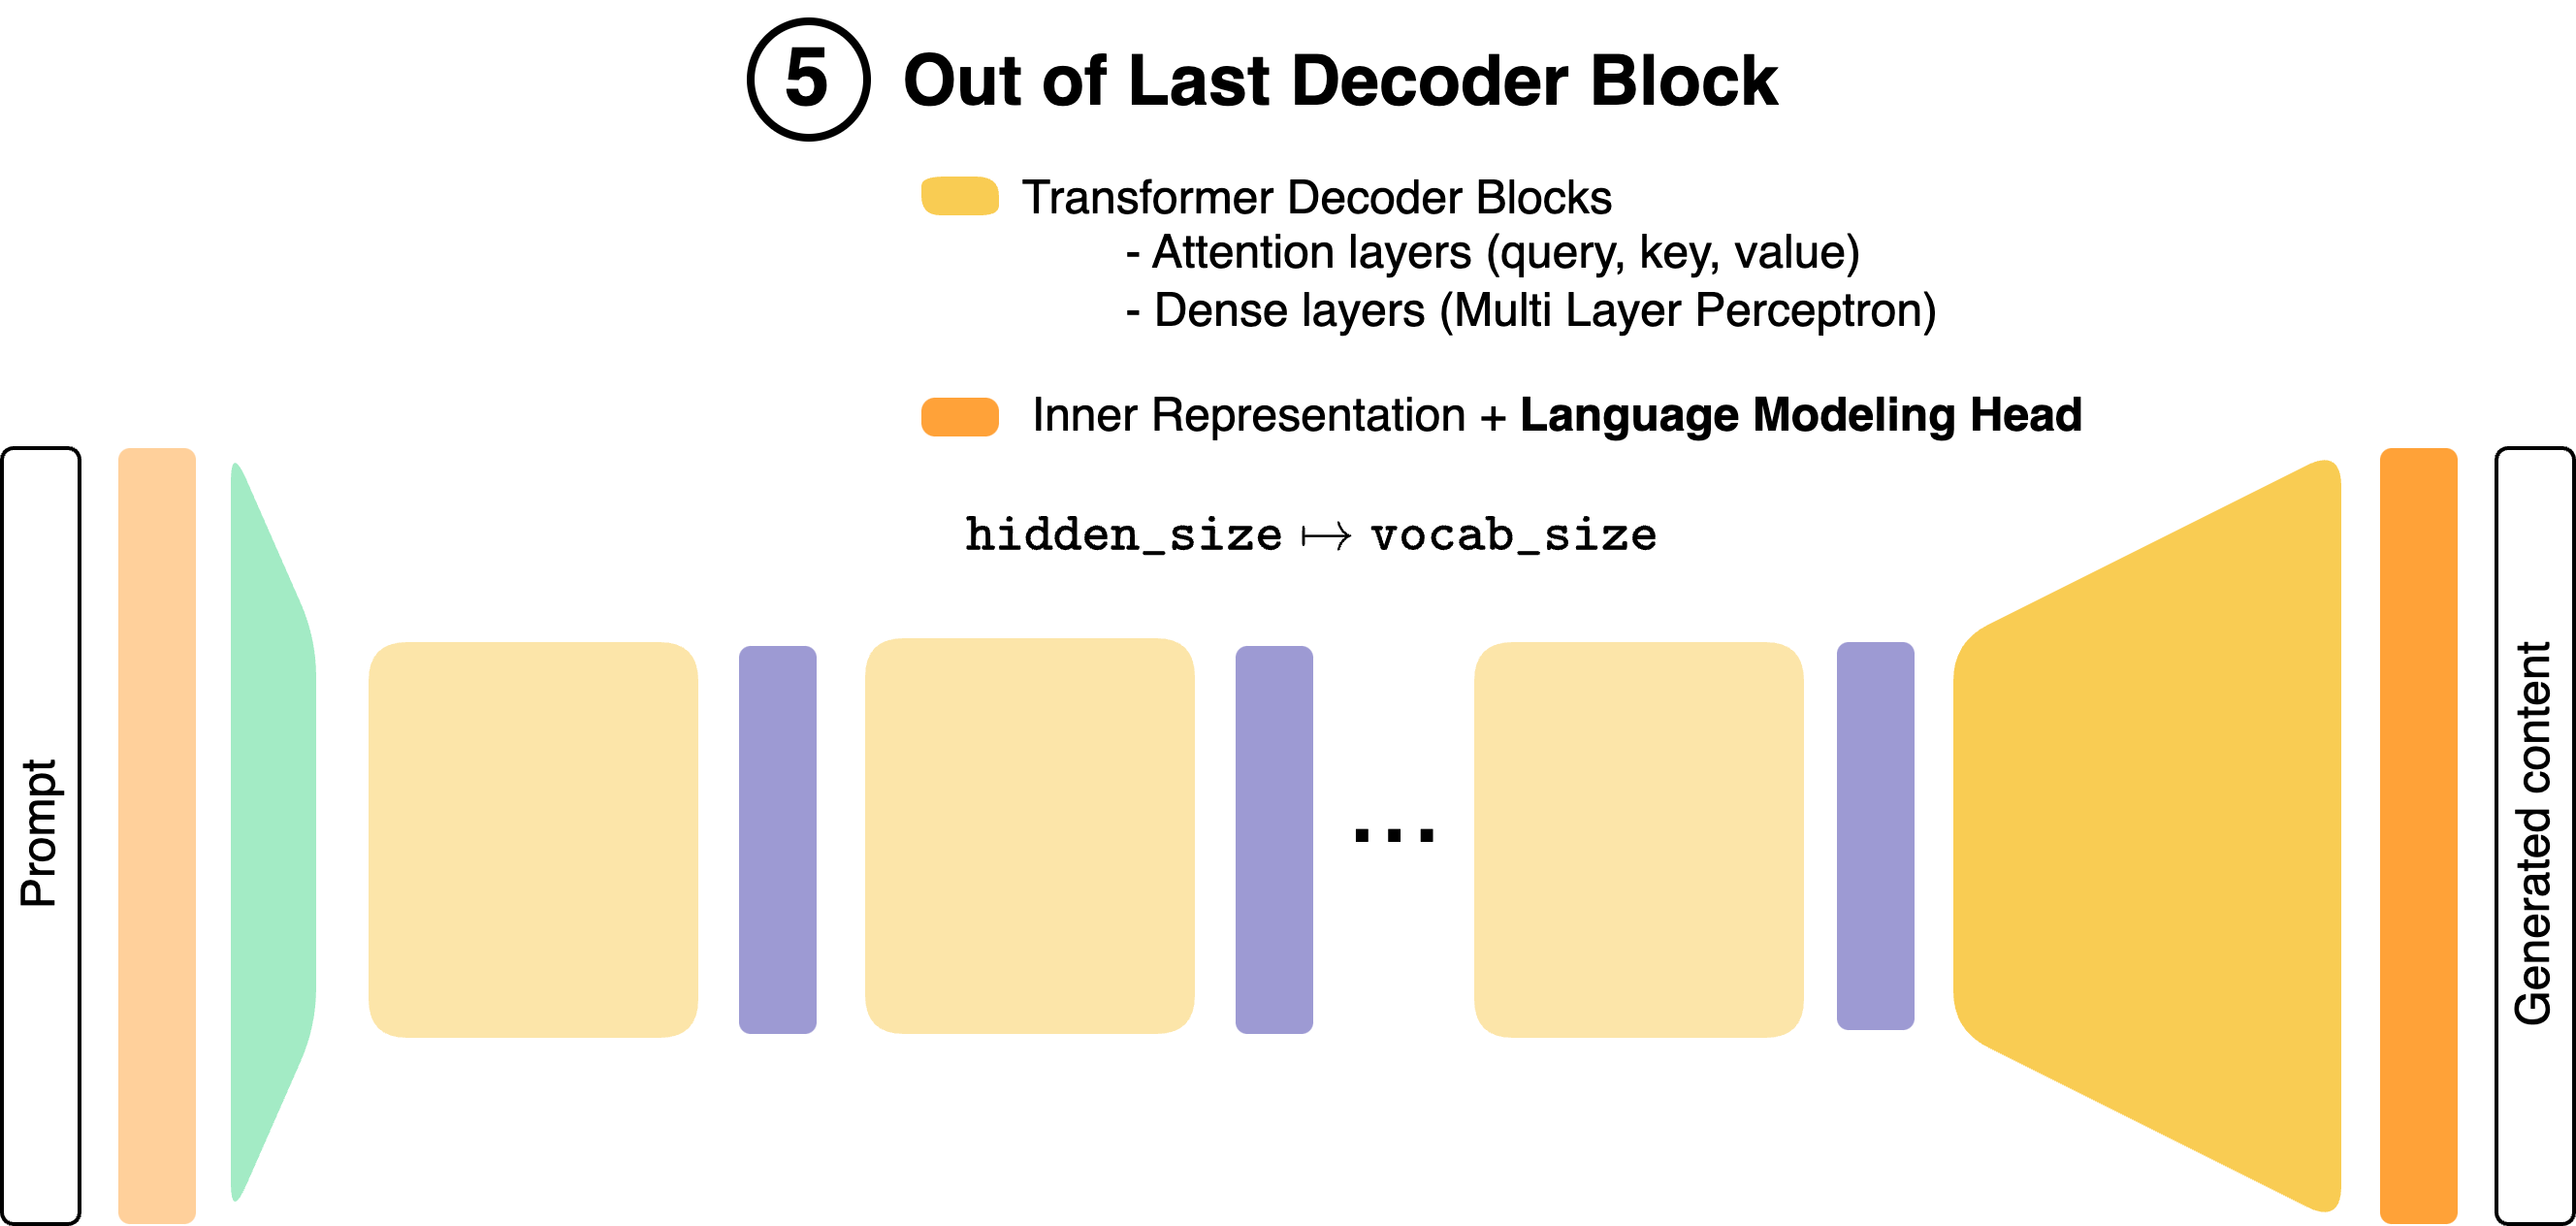
\includegraphics[width=0.95\textwidth]{llm_8.png}
    \end{figure}
\end{frame}

\begin{frame}{Inside a Decoder-Based LLM}
    \begin{figure}
        \centering
        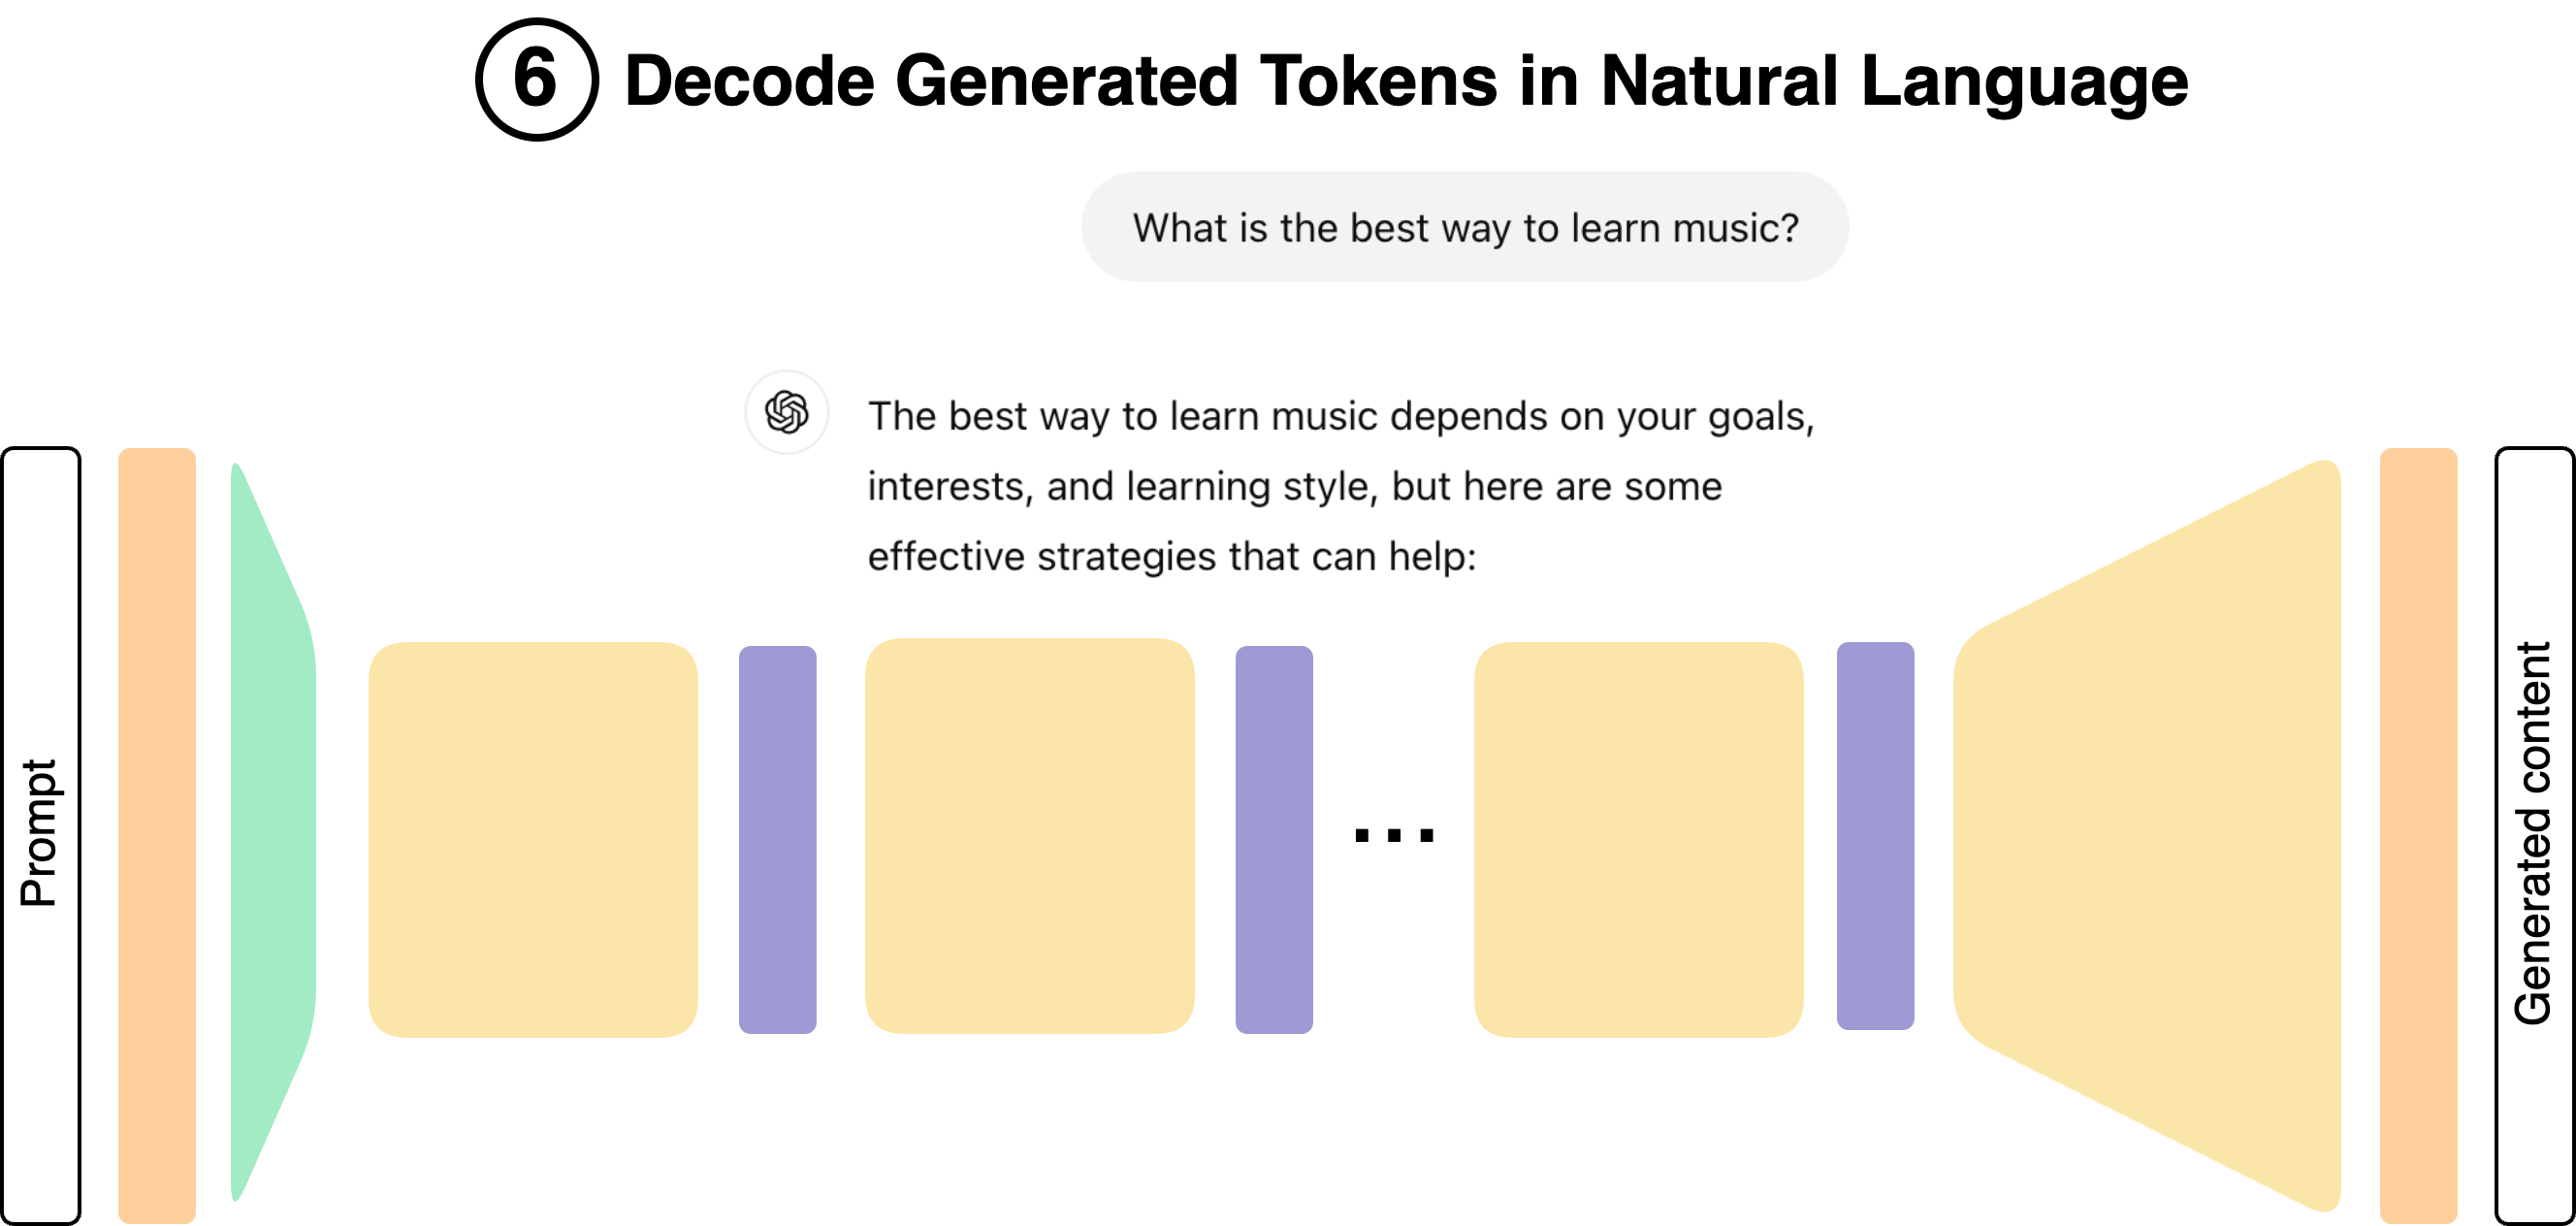
\includegraphics[width=0.95\textwidth]{llm_9.png}
    \end{figure}
\end{frame}

\begin{frame}{The Autoregressive Principle}
    \begin{figure}
        \centering
        \includegraphics[width=0.95\textwidth]{llm_autoregressive_1.png}
    \end{figure}
\end{frame}

\begin{frame}{The Autoregressive Principle}
    \begin{figure}
        \centering
        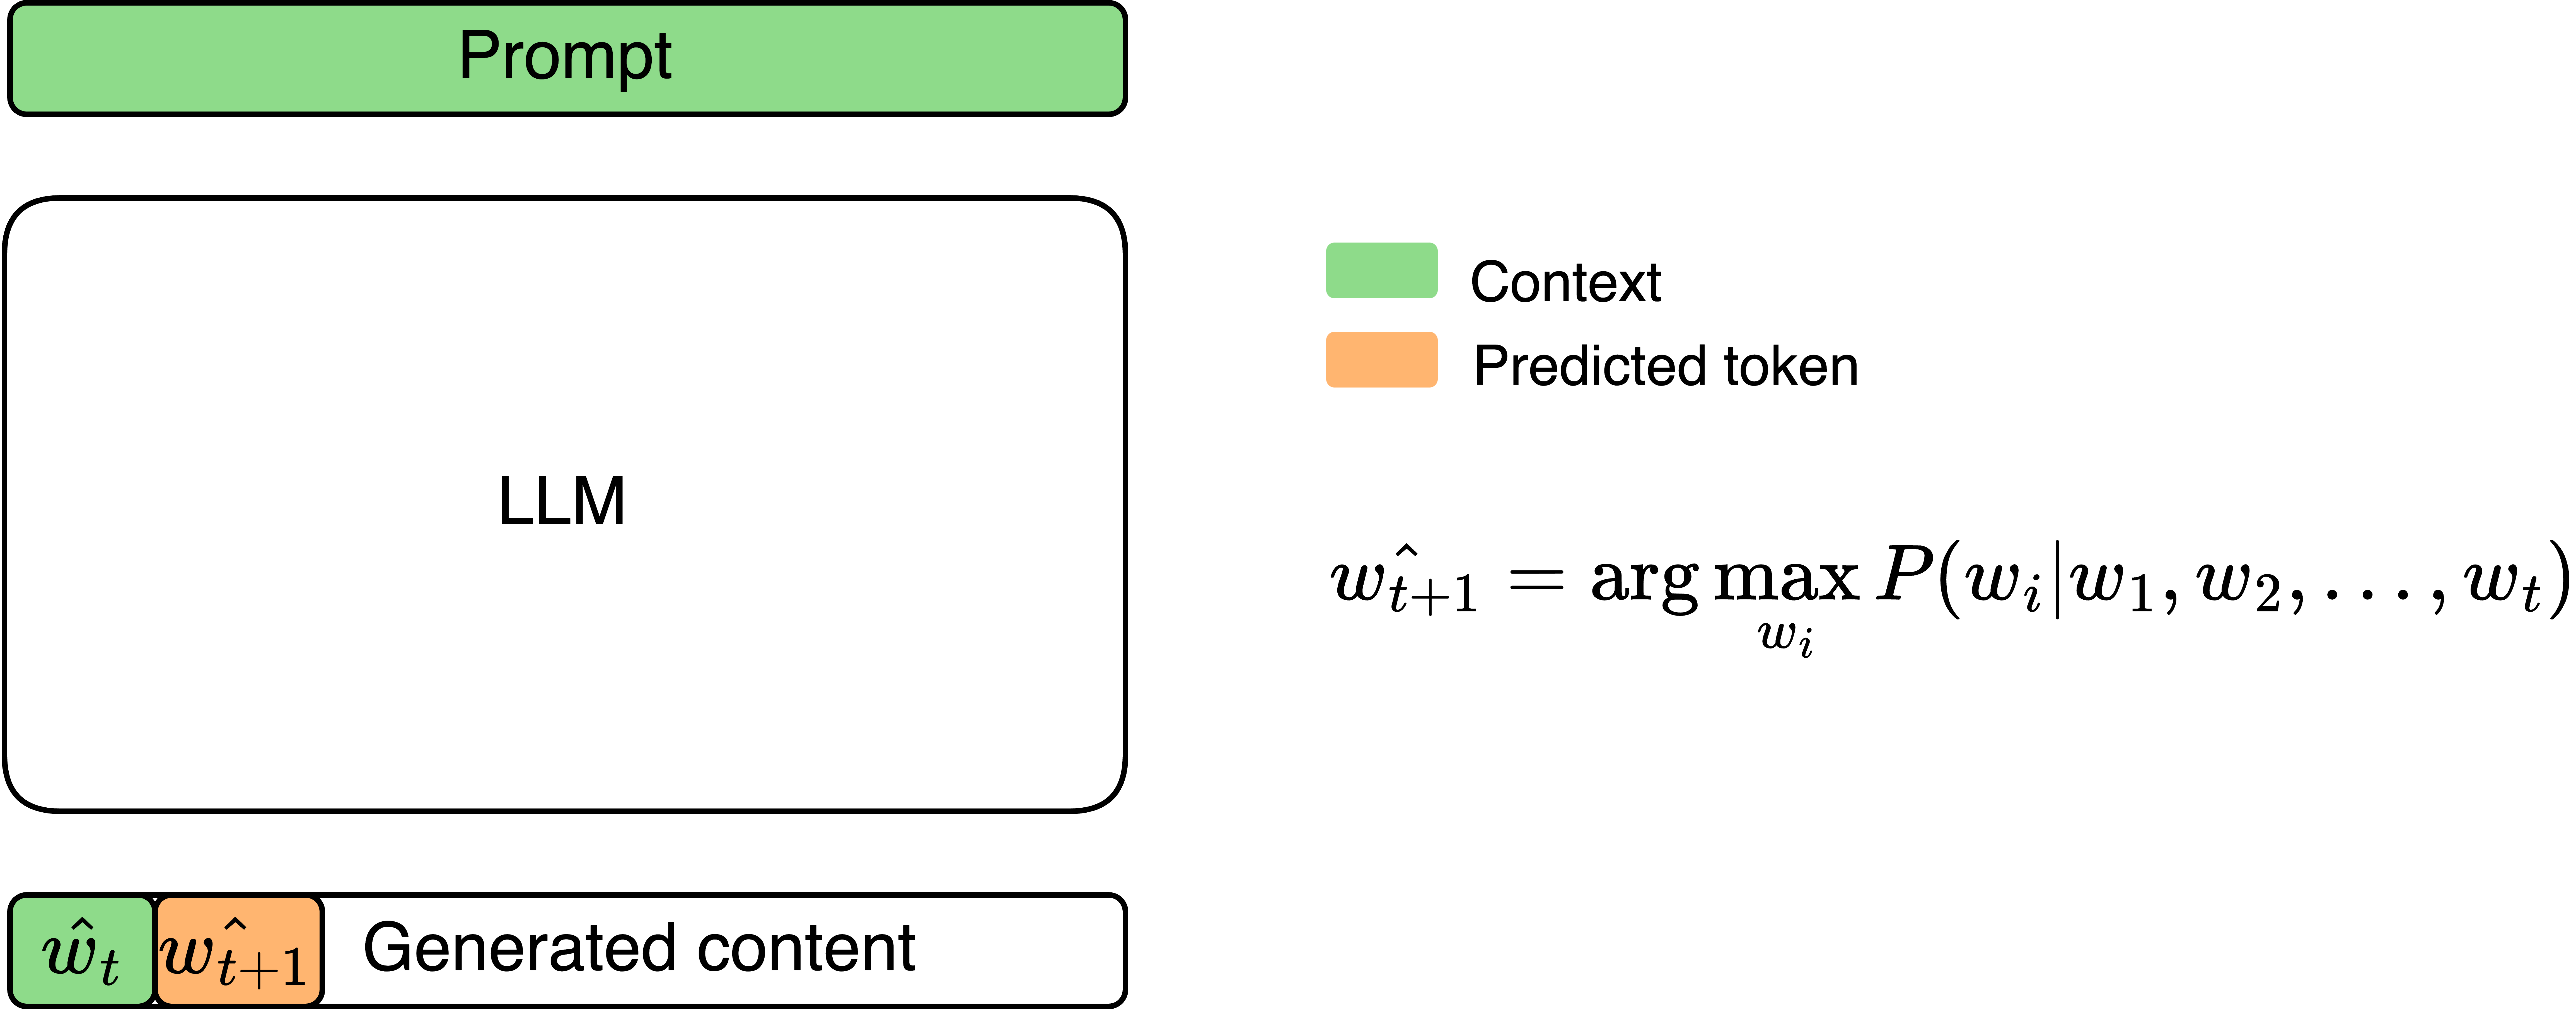
\includegraphics[width=0.95\textwidth]{llm_autoregressive_2.png}
    \end{figure}
\end{frame}

% - Petit point d'étape, prise de recul. Déjà, "Large" comment ("How large and Large Language Models?")
%     - Donner des valeurs chiffrées pour donner des repères aux gens, ainsi que des temps d'exécution indicatifs et les requirements CPU/GPU pour faire des choses classiques. Ne présenter que les LLMs open-source et en profiter pour dire que les modèles type GPT, Claude etc. sont closed-source donc on ne sait pas
%     - Autre point de détail au passage: open-source / open-weight ("Open-source or open-weights?")
% - Paradigme pré-entraînement / affinage, parallèle fromage
%     - On arrive à la problématique du fine-tuning
% - Comment faire un fine-tuning efficace?
%     - On a vu le temps que ça prenait de mettre à jour tous les paramètres donc on n'a pas envie de faire ça
%     - Ne mettre à jour que certains paramètres : comment les choisir ? 
%     - Adapters, Low-Rank Adaptation
%         - Explication du concept des adapters
%         - Description du principe de LoRA
%         - Présentation d'adapters hub (bien préciser que les adapters sont modèle dépendants)


\end{document}